\documentclass[../main.tex]{subfiles}
\begin{document}
\paragraph{Online solutions}\label{par:conservation_rom}

Just as in problem $2.$ for the parabolic case, here the reduced order system preserves time-dependence.
The transient FOM and ROM solutions are compared in Figure \ref{fig:conservation_rom}

\begin{figure}[H]
    \centering 
    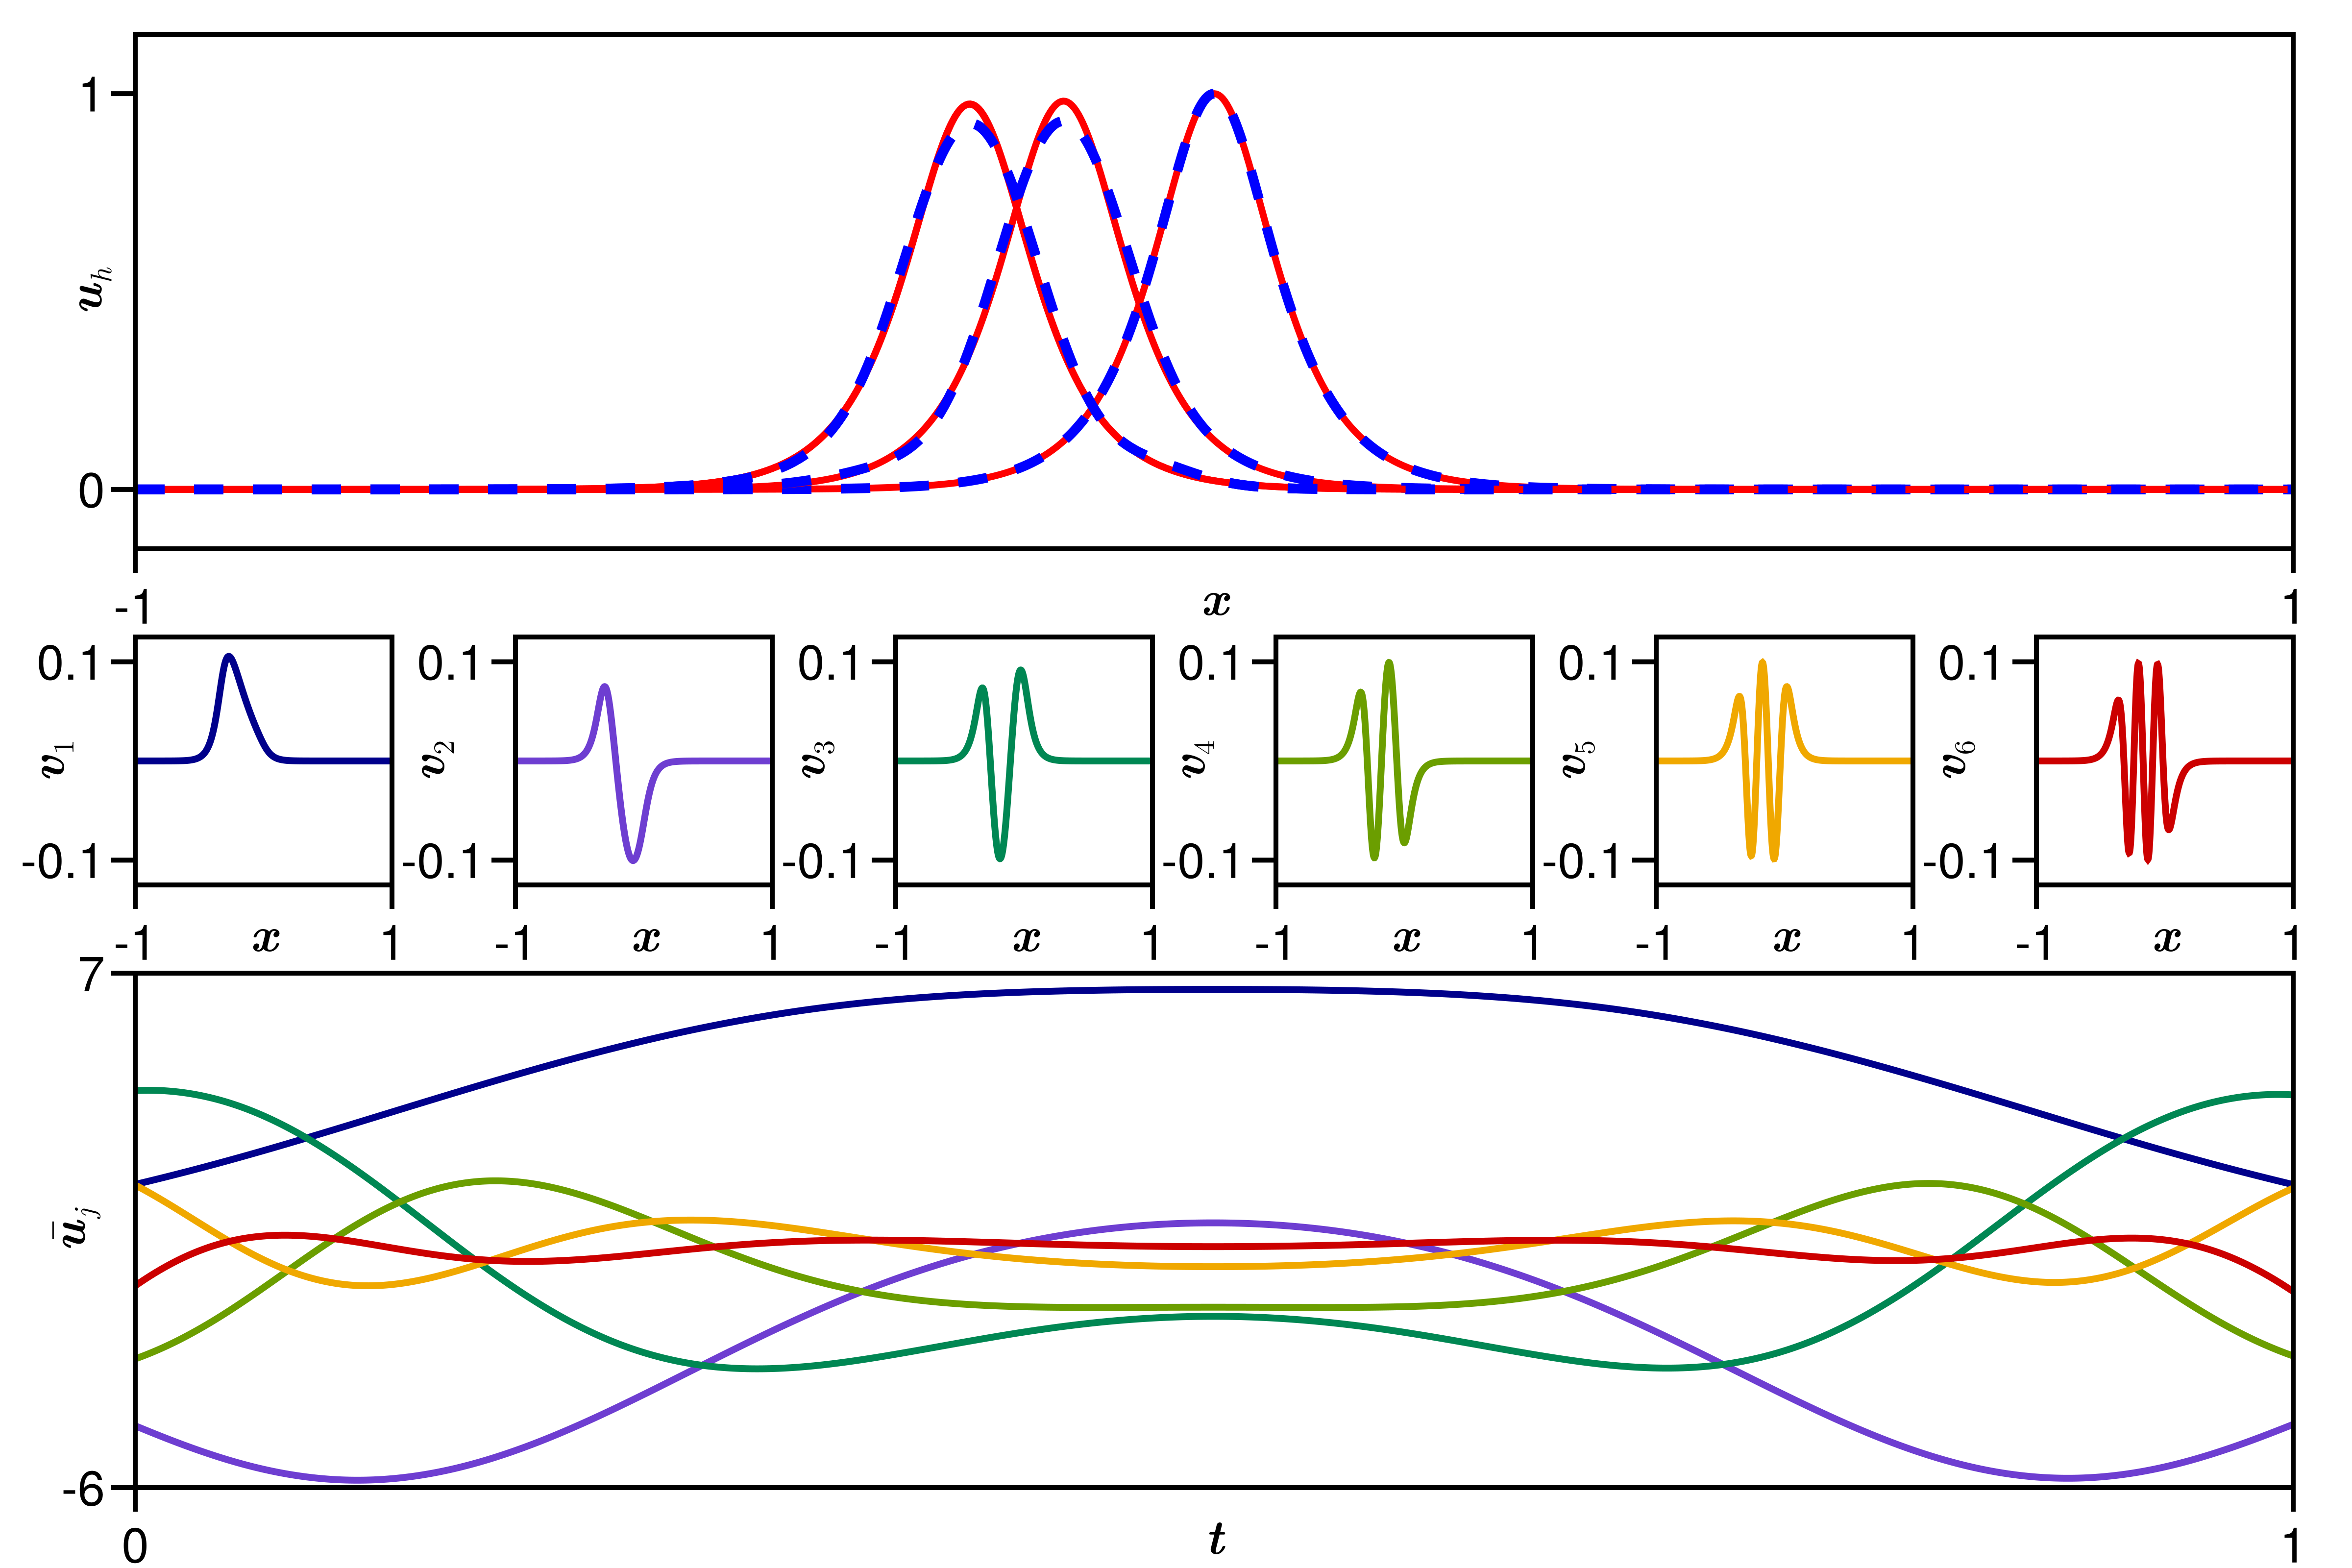
\includegraphics[keepaspectratio, width=0.75\textwidth]{../figures/fig:conservation_rom.png}
    \caption{\textbf{Top}: comparison of some solutions of the FOM (solid, red) and the ROM (dashed, blue) for parameter value $\mu = 0.75$.
             \textbf{Middle}: first $6$ singular vectors of the SVD of the snapshot matrix and basis functions of the ROM.
     \textbf{Bottom}: time-evolution of the coefficients of the affine expansion \eqref{eq:ansatz} of the reduced dynamical system.
     These are color coded to match the basis function to which they are associated.
}
    \label{fig:conservation_rom}
\end{figure}

The ROM well captures the time-evolution of the FOM however it requires $6$ modes of the SVD of the snapshot matrix to retain the $99\%$ accuracy treshold we specified.
This is quite a substantial increase from the elliptic and both the steady-state and time-dependent problems of the parabolic cases we investigated earlier, where at most $2$ basis functions were needed.
While the Kolmogoroff $n-$width decay is still exponential (see Figure \ref{fig:conservation_decay}) it is considerably slower in the hyperbolic case than the previous two

\begin{figure}[H]
    \centering 
    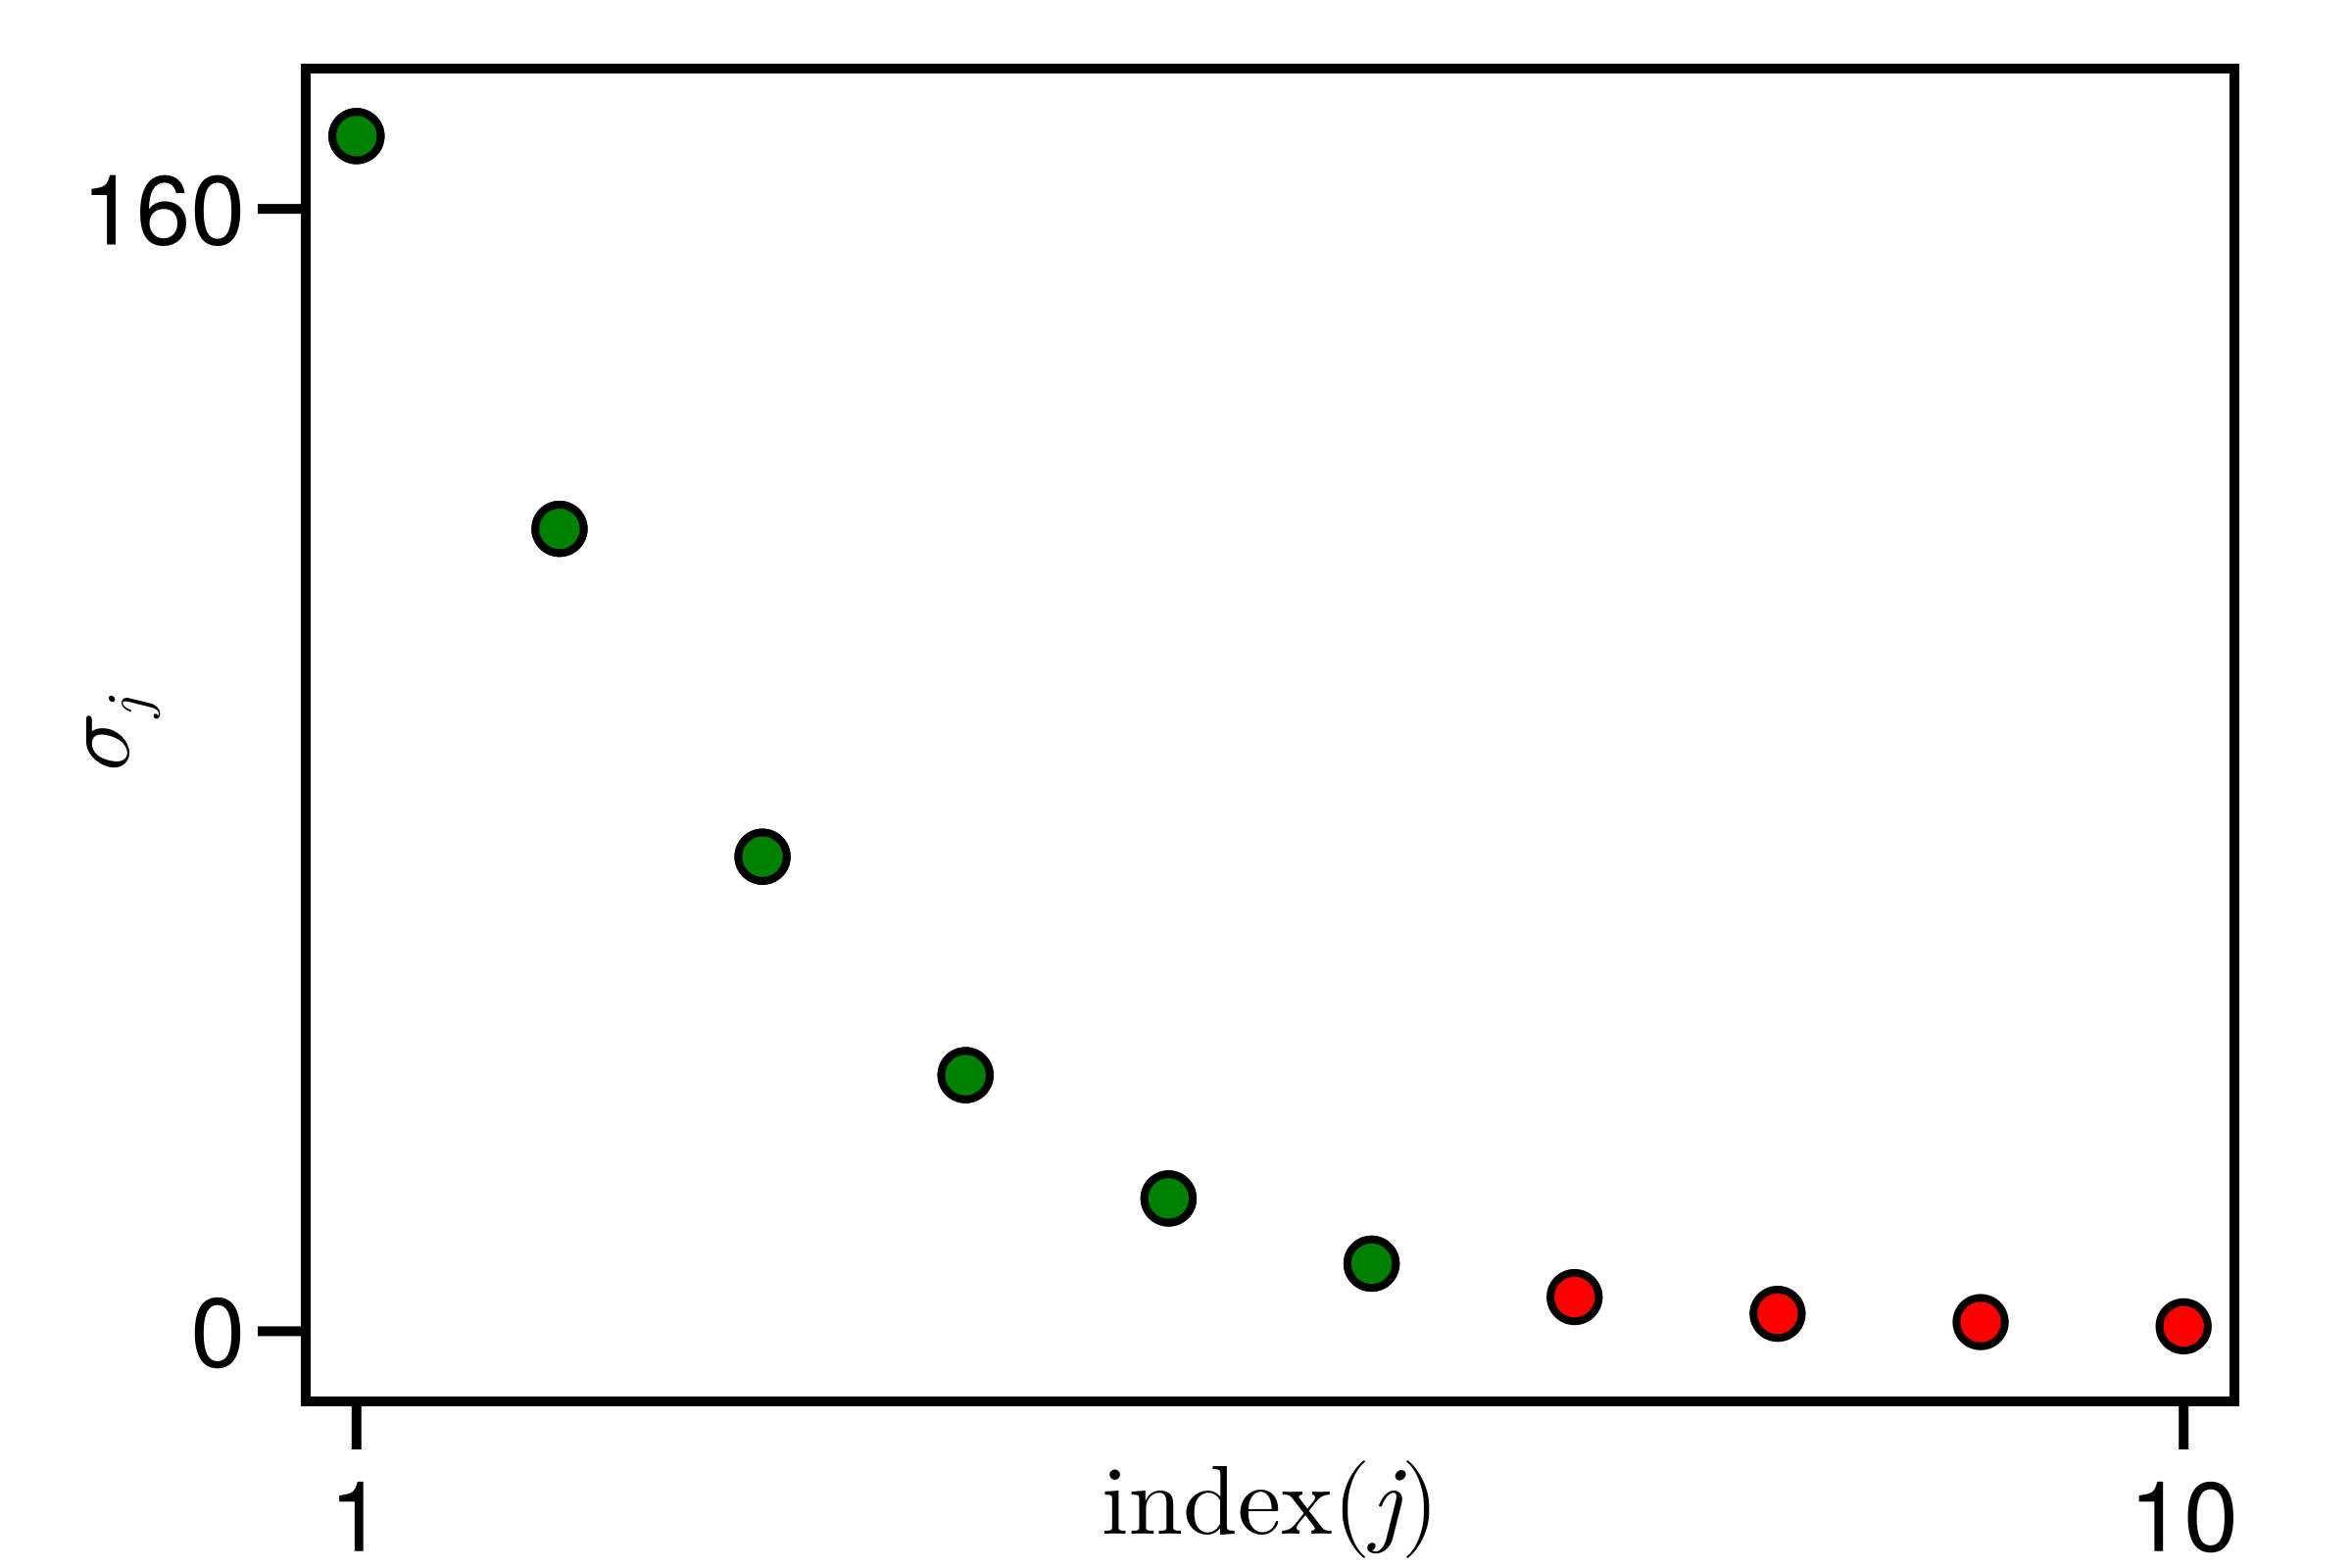
\includegraphics[keepaspectratio, width=0.7\textwidth]{../figures/fig:conservation_decay.png}
    \caption{Kolmogoroff $n-$width decay of \eqref{eq:conservation}. Green dots reppresent the $N_{r}=6$ singular values used for constructing $\mathcal{R}_{h}$.}
    \label{fig:conservation_decay}
\end{figure}

\end{document}
